%
% funktionen.tex -- Neue Funktionen: elliptische Integrale und Funktionen
%
% (c) 2026 Baris Catan, OST Ostschweizer Fachhochschule
%
% !TEX root = ../../buch.tex
% !TEX encoding = UTF-8
%
\section{Neue Funktionen
\label{elliptisch:section:funktionen}}
\kopfrechts{Neue Funktionen}

Im vorherigen Abschnitt ist das Umfangsintegral
\eqref{elliptisch:equation:umfang} als elliptisches Integral ohne
elementare Stammfunktion eingeordnet worden.
Die Definition \eqref{elliptisch:equation:definition} lässt für die
rationale Funktion $R$ und das Polynom $p$ unendlich viele
Möglichkeiten zu, und für jede davon eine eigene Funktion
einzuführen wäre unpraktisch und, wie sich zeigen wird, auch gar
nicht nötig.

\subsection{Der Reduktionssatz}
Die elliptischen Integrale bilden zwar eine unübersehbare Menge,
aber sie unterscheiden sich nur um elementare Anteile, und was
davon übrig bleibt, sind drei feste Integrale.
\begin{satz}[Reduktionssatz]
\label{elliptisch:satz:reduktion}
Jedes elliptische Integral lässt sich als Summe elementarer
Funktionen und der drei Integrale
\begin{equation}
\int \frac{dt}{\sqrt{p(t)}},
\qquad
\int \frac{\sqrt{1-k^2t^2}}{\sqrt{1-t^2}}\,dt,
\qquad
\int \frac{dt}{(1-nt^2)\sqrt{p(t)}}
\label{elliptisch:equation:normalformen}
\end{equation}
mit dem Polynom $p(t) = (1-t^2)(1-k^2t^2)$ unter der Wurzel,
$0 < k < 1$ und $n \in \mathbb{R}$ schreiben.
\end{satz}
Der Beweis ist bei Smirnow zu finden
\cite[Abschnitt~164, S.~506]{elliptisch:smirnow} und \cite{elliptisch:mueller-spezielle}.
Er verläuft in zwei Schritten.
Zuerst wird das beliebige Polynom $p$ vom Grad $3$ oder $4$ durch
eine gebrochen lineare Substitution auf die Form
$(1-t^2)(1-k^2t^2)$ unter der Wurzel gebracht, was den Modul $k$
überhaupt erst erzeugt.
Danach wird der rationale Anteil des Integranden durch
Partialbruchzerlegung und wiederholte partielle Integration
abgebaut, bis nur noch die drei Reste in
\eqref{elliptisch:equation:normalformen} stehen.
\index{Reduktionssatz}%

Diese drei heissen elliptische Integrale erster, zweiter und
dritter Art.
Die Zahl $k$ heisst \emph{Modul}, die Zahl $n$ in der dritten Art
\emph{Charakteristik}.
\index{Modul}%
\index{Charakteristik}%
Schreibt man das Integral zweiter Art stattdessen über dem
gemeinsamen Nenner $\sqrt{p(t)}$, kürzt sich ein Faktor
$\sqrt{1-k^2t^2}$ heraus und man erhält wieder die Form aus
\eqref{elliptisch:equation:normalformen},
\begin{equation}
\int \frac{1-k^2t^2}{\sqrt{p(t)}}\,dt
=
\int \frac{1-k^2t^2}{\sqrt{(1-t^2)(1-k^2t^2)}}\,dt
=
\int \frac{\sqrt{1-k^2t^2}}{\sqrt{1-t^2}}\,dt
=
\int \sqrt{\frac{1-k^2t^2}{1-t^2}}\,dt.
\label{elliptisch:equation:zweiteart}
\end{equation}
Alle drei Arten haben damit dasselbe Polynom unter der Wurzel, sie
unterscheiden sich nur im Zähler und im zusätzlichen Faktor
$1-nt^2$.

Eine Warnung zur Notation ist hier angebracht.
Viele Tabellenwerke und Programmbibliotheken benutzen statt des
Moduls $k$ den Parameter $m = k^2$.
In \texttt{scipy} etwa liefert erst \texttt{ellipk(k**2)} das
Integral zum Modul $k$.
Wir schreiben durchgehend $k$.

\subsection{Die vollständigen elliptischen Integrale}
Die Integrale in \eqref{elliptisch:equation:normalformen} sind
unbestimmt und legen damit keine Funktion fest.
Eine Funktion entsteht erst, wenn wir die Grenzen festsetzen.
Das Polynom $p(t)$ unter der Wurzel hat bei $t = \pm 1$ eine
Nullstelle, weiter als bis $1$ lässt sich also nicht integrieren.
Genau diese Grenzen wählen wir.
\begin{definition}
\label{elliptisch:definition:vollstaendig}
Die vollständigen elliptischen Integrale erster, zweiter und
dritter Art sind für $0 < k < 1$ und $n \in \mathbb{R}$
\begin{equation}
\begin{aligned}
K(k)
&=
\int_0^1 \frac{dt}{\sqrt{(1-t^2)(1-k^2t^2)}},
\\
E(k)
&=
\int_0^1 \sqrt{\frac{1-k^2t^2}{1-t^2}}\,dt,
\\
\Pi(n,k)
&=
\int_0^1 \frac{dt}{(1-nt^2)\sqrt{(1-t^2)(1-k^2t^2)}}.
\end{aligned}
\label{elliptisch:equation:vollstaendig}
\end{equation}
\end{definition}
\index{elliptisches Integral!vollstandiges@vollständiges}%
\index{K@$K(k)$}%
\index{E@$E(k)$}%
Für die Anwendungen in
Abschnitt~\ref{elliptisch:section:anwendungen} genügen die ersten
beiden Arten, die dritte Art entsteht erst, wenn der Nenner des
rationalen Anteils Nullstellen mitbringt.

Diese Schreibweise heisst \emph{Jacobi-Normalform}.
Die Substitution $t = \sin\varphi$ führt auf eine zweite
gebräuchliche Form.
Wegen $\sqrt{1-t^2} = \cos\varphi$ und $dt = \cos\varphi\,d\varphi$
ist
\begin{equation}
\frac{dt}{\sqrt{1-t^2}}
=
d\varphi,
\label{elliptisch:equation:legendresubst}
\end{equation}
und die obere Grenze $t = 1$ geht in $\varphi = \pi/2$ über.
Damit werden aus \eqref{elliptisch:equation:vollstaendig} die
Integrale
\begin{equation}
K(k)
=
\int_0^{\pi/2} \frac{d\varphi}{\sqrt{1-k^2\sin^2\varphi}},
\qquad
E(k)
=
\int_0^{\pi/2} \sqrt{1-k^2\sin^2\varphi}\,d\varphi,
\label{elliptisch:equation:legendreform}
\end{equation}
und entsprechend für $\Pi$.
Diese Schreibweise heisst \emph{Legendre-Normalform}
\cite[Abschnitt 11.1.2]{elliptisch:mueller-spezielle}.
\index{Jacobi-Normalform}%
\index{Legendre-Normalform}%
Beide Formen beschreiben dieselben Funktionen.
Wer in der Literatur einmal die obere Grenze $1$ und einmal
$\pi/2$ antrifft, kennt nun die Beziehung zwischen beiden Formen.

\subsection{Randwerte und Verlauf}
$K$ und $E$ hängen stetig von $k$ ab und an beiden Rändern des
Intervalls $0 < k < 1$ lassen sich die Werte direkt ausrechnen.
Für $k = 0$ verschwindet der Term mit $k^2$ in beiden Integralen,
und es bleibt zweimal dasselbe stehen,
\begin{equation}
K(0)
=
E(0)
=
\int_0^1 \frac{dt}{\sqrt{1-t^2}}
=
\arcsin 1
=
\frac{\pi}{2}.
\label{elliptisch:equation:randnull}
\end{equation}
Das ist der Viertelkreis, wie schon in der Einleitung gesehen.
Für $k = 1$ trennen sich die beiden.
Beim Integral zweiter Art kürzen sich Zähler und Nenner vollständig,
\begin{equation}
E(1)
=
\int_0^1 \sqrt{\frac{1-t^2}{1-t^2}}\,dt
=
\int_0^1 dt
=
1.
\label{elliptisch:equation:randeins}
\end{equation}
Beim Integral erster Art dagegen wird das Polynom unter der Wurzel
zu $(1-t^2)^2$, der Integrand also zu
\begin{equation}
\frac{1}{1-t^2}
\approx
\frac{1}{2(1-t)}
\qquad
\text{für } t \to 1,
\label{elliptisch:equation:kdivergenz}
\end{equation}
und $\int^1 dt/(1-t)$ divergiert logarithmisch.
Somit ist $K(1) = \infty$.
Wie schnell $K$ wächst, beschreibt man am besten mit dem
\emph{komplementären Modul}
\begin{equation}
k' = \sqrt{1-k^2},
\qquad
k^2 + k'^2 = 1,
\label{elliptisch:equation:kstrich}
\end{equation}
\index{Modul!komplementarer@komplementärer}%
der den Abstand zum Fall $k = 1$ misst.
Mit ihm gilt die Asymptotik
\begin{equation}
K(k)
\sim
\log \frac{4}{k'}
\qquad
\text{für } k \to 1
\label{elliptisch:equation:kasymptotik}
\end{equation}
\cite[Abschnitt~11.1]{elliptisch:mueller-spezielle}.
Abbildung~\ref{fig:elliptisch:keplot} zeigt beide Funktionen.
\begin{figure}
	\centering
	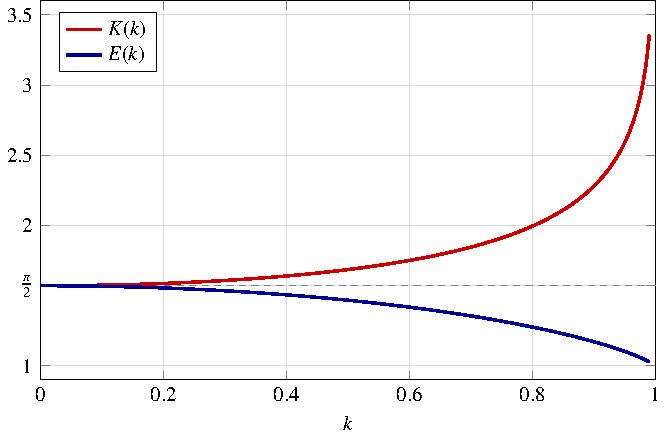
\includegraphics[width=0.72\textwidth]{papers/elliptisch/images/ke-plot.pdf}
	\caption{Die vollständigen elliptischen Integrale erster und
	zweiter Art.
	Beide starten bei $k=0$ im gemeinsamen Wert $\pi/2$.
	$E(k)$ fällt monoton auf $E(1) = 1$, während $K(k)$ monoton wächst
	und für $k \to 1$ logarithmisch divergiert.}
	\label{fig:elliptisch:keplot}
\end{figure}


\subsection{Der Ellipsenumfang mit $E(k)$
\label{elliptisch:subsection:ellipsenumfangE}}
Der Vergleich von \eqref{elliptisch:equation:legendreform} mit dem
Umfangsintegral \eqref{elliptisch:equation:umfang} zeigt, dass wir
die gesuchte Funktion bereits haben.
Das Integral zweiter Art in Legendre-Normalform ist Zeichen für
Zeichen der Ausdruck, der beim Ellipsenumfang stehen geblieben ist,
und damit gilt
\begin{equation}
U
=
4a\,E(k),
\qquad
k^2 = \frac{a^2-b^2}{a^2},
\qquad
a \ge b.
\label{elliptisch:equation:umfangE}
\end{equation}
Für den Kreis ist $k = 0$ und mit $E(0) = \pi/2$ folgt
$U = 4a\cdot\pi/2 = 2\pi a$.
Die Frage vom Anfang des Kapitels ist damit beantwortet, wenn auch
nicht durch eine elementare Formel, sondern durch eine eigens
definierte Funktion.
Dabei ist die Reihenfolge das Entscheidende.
Auch $\int dt/t$ war nicht darstellbar, solange es den Logarithmus
noch nicht gab, und erst seine Aufnahme in den Funktionsvorrat hat
das Integral lösbar gemacht.
Elementar ist also keine Eigenschaft eines Integrals an sich,
sondern eine Aussage über einen vorher festgelegten Vorrat.

\subsection{Unvollständige Integrale und Umkehrung
\label{elliptisch:subsection:unvollstaendig}}
Die vollständigen Integrale \eqref{elliptisch:equation:vollstaendig}
hängen nur von den Parametern $k$ und $n$ ab.
Funktionen der oberen Grenze entstehen, wenn wir sie variabel
machen.
\begin{definition}
\label{elliptisch:definition:unvollstaendig}
Die \emph{unvollständigen elliptischen Integrale} entstehen aus
den vollständigen, indem die obere Grenze $1$ durch die Variable
$x$ mit $0 \le x \le 1$ ersetzt wird,
\begin{equation}
\begin{aligned}
F(x,k)
&=
\int_0^x \frac{dt}{\sqrt{(1-t^2)(1-k^2t^2)}},
\\
E(x,k)
&=
\int_0^x \sqrt{\frac{1-k^2t^2}{1-t^2}}\,dt,
\\
\Pi(n,x,k)
&=
\int_0^x \frac{dt}{(1-nt^2)\sqrt{(1-t^2)(1-k^2t^2)}}.
\end{aligned}
\label{elliptisch:equation:unvollstaendig}
\end{equation}
\end{definition}
\index{elliptisches Integral!unvollstandiges@unvollständiges}%
Die Namen sind dieselben wie bei den vollständigen Integralen,
die Anzahl der Argumente unterscheidet die beiden Fassungen.
Zwei Spezialfälle halten wir fest.
An der oberen Grenze $x = 1$ wird aus dem unvollständigen
Integral wieder das vollständige, es ist $F(1,k) = K(k)$, und
entsprechend für die beiden anderen Arten.
Für $k = 0$ bleibt nur das Arcussinus-Integral stehen,
\begin{equation}
F(x,0)
=
E(x,0)
=
\int_0^x \frac{dt}{\sqrt{1-t^2}}
=
\arcsin x.
\label{elliptisch:equation:knullarcsin}
\end{equation}

Diese Zeile ist der Schlüssel zum nächsten Schritt.
Sie besagt, dass die Umkehrfunktion von $F(\,\cdot\,, 0)$ der
Sinus ist.
Dieselbe Geste, angewendet auf beliebiges $k$, liefert
\begin{equation}
\begin{aligned}
s
&=
\arcsin x
&\quad&\Leftrightarrow\quad&
x
&=
\sin s,
\\
u
&=
F(x,k)
&\quad&\Leftrightarrow\quad&
x
&=
\operatorname{sn}(u,k).
\end{aligned}
\label{elliptisch:equation:umkehrung}
\end{equation}
Die untere Zeile ist die Definition des
\emph{sinus amplitudinis} $\operatorname{sn}(u,k)$.
Weil der Integrand von $F$ positiv ist, wächst
$F(\,\cdot\,, k)$ streng monoton von $0$ auf $K(k)$, wenn $x$ das
Intervall $[0,1]$ durchläuft.
Die Umkehrfunktion existiert also und ist zunächst auf
$[0, K(k)]$ erklärt, definitionsgemäss gilt
$F(\operatorname{sn}(u,k), k) = u$.
\index{sn@$\operatorname{sn}(u,k)$}%

Den Namen erklärt die Legendre-Normalform.
Mit $x = \sin\varphi$ geht $u = F(x,k)$ in
\begin{equation}
u
=
\int_0^\varphi \frac{d\vartheta}{\sqrt{1-k^2\sin^2\vartheta}}
\label{elliptisch:equation:amplitude}
\end{equation}
über, und das Auflösen dieser Beziehung nach $\varphi$ liefert die
sogenannte \emph{Amplitude} $\varphi = \operatorname{am}(u,k)$.
Damit ist $\operatorname{sn}(u,k) = \sin\operatorname{am}(u,k)$,
der Sinus der Amplitude, also genau das, was der Name sagt.
\index{Amplitude}%

Die Bezeichnung \emph{sinus amplitudinis} stammt von Jacobi und
erklärt die Abkürzung $\operatorname{sn}$
\cite[Abschnitt~11.2]{elliptisch:mueller-spezielle}.
Der Schritt zur Umkehrung ist auch historisch der entscheidende.
Die elliptischen Integrale sind lange untersucht und tabelliert
worden, vor allem von Legendre.
Den \emph{Durchbruch} brachte erst ihre Umkehrung durch Abel und Jacobi,
mit der die elliptischen Funktionen entstanden sind.
1827 bewies Jacobi mit diesem Schritt seine allgemeine
Transformationsformel
\cite{elliptisch:wiki-elliptische-funktion}.
Was die neue Funktion mit dem Sinus gemeinsam hat und worin sie
sich von ihm unterscheidet, zeigt der nächste Abschnitt.

\subsection{Die geometrische Gestalt von sn, cn und dn
\label{elliptisch:subsection:geometrie}}
Was für den Sinus der Einheitskreis ist, ist für
$\operatorname{sn}$ eine Ellipse.
Der Einheitskreis fasst die Kreisfunktionen zusammen.
Sein Punkt, dessen Bogenlänge vom Punkt $(1,0)$ aus $u$ beträgt,
hat die Koordinaten $(\cos u, \sin u)$
(Abbildung~\ref{fig:elliptisch:snkonstruktion} links).
Auf der Ellipse mit den Halbachsen $a \ge 1$ und $1$,
\begin{equation}
\frac{x^2}{a^2} + y^2 = 1,
\label{elliptisch:equation:einheitsellipse}
\end{equation}
hängen Winkel, Bogenlänge und Koordinaten nicht mehr so einfach
zusammen.
Wir schreiben einen Punkt der Ellipse mit dem Hilfswinkel
$\varphi$ als
\begin{equation}
P
=
(a\cos\varphi, \sin\varphi)
\label{elliptisch:equation:ellipsenpunkt}
\end{equation}
und messen seine Lage durch den Parameter $u$ aus
\eqref{elliptisch:equation:amplitude}, sodass
$\varphi = \operatorname{am}(u,k)$ ist, mit dem Modul
$k = \sqrt{a^2-1}/a$.
Die drei jacobischen Funktionen sind die
Koordinatenverhältnisse dieses Punktes,
\begin{equation}
\operatorname{sn}(u,k) = y,
\qquad
\operatorname{cn}(u,k) = \frac{x}{a},
\qquad
\operatorname{dn}(u,k) = \frac{r}{a},
\qquad
r = \sqrt{x^2+y^2}.
\label{elliptisch:equation:geometrischedefinition}
\end{equation}
Die ersten beiden besagen
$\operatorname{sn}(u,k) = \sin\varphi = \sin\operatorname{am}(u,k)$
und $\operatorname{cn}(u,k) = \cos\varphi$, genau die Umkehrung
aus Abschnitt~\ref{elliptisch:subsection:unvollstaendig}.
Der gestrichelte Hilfskreis in
Abbildung~\ref{fig:elliptisch:snkonstruktion} trägt den Punkt
$Q = (\operatorname{cn}(u,k), \operatorname{sn}(u,k))$, an dem
sich der Winkel $\varphi$ ablesen lässt.
Für die dritte rechnet man $r^2 = a^2\cos^2\varphi + \sin^2\varphi$
nach und findet
\begin{equation}
\operatorname{dn}(u,k)^2
=
\frac{r^2}{a^2}
=
1 - k^2\sin^2\varphi
=
1 - k^2\operatorname{sn}(u,k)^2.
\label{elliptisch:equation:dngeometrie}
\end{equation}
\begin{figure}
	\centering
	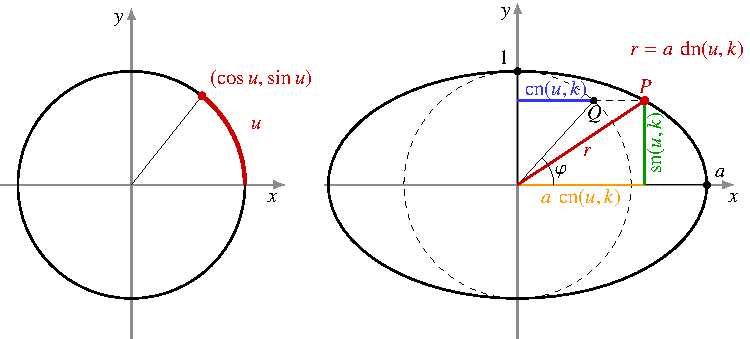
\includegraphics[width=\textwidth]{papers/elliptisch/images/sn-konstruktion.pdf}
	\caption{Links der Einheitskreis mit dem Punkt $(\cos u, \sin u)$
	zur Bogenlänge $u$.
	Rechts die Ellipse mit den Halbachsen $a = 1/k'$ und $1$ zum
	selben Parameter, hier $u = 0.9$ und $k = 0.8$.
	Die Punkte
	$Q = (\operatorname{cn}(u,k), \operatorname{sn}(u,k))$
	und
	$P = (a\operatorname{cn}(u,k), \operatorname{sn}(u,k))$
	liegen auf gleicher Höhe, der Abstand von $P$ zum Nullpunkt ist
	$r = a\operatorname{dn}(u,k)$.
	Nach \cite[Abschnitt~11.2.1]{elliptisch:mueller-spezielle} und
	\cite{elliptisch:schwalm}.}
	\label{fig:elliptisch:snkonstruktion}
\end{figure}


Der Parameter $u$ ist weder der Winkel $\varphi$ noch die
Bogenlänge der Ellipse.
Nur im Kreisfall $k = 0$ fallen alle drei zusammen.
Dann ist $a = 1$, die Ellipse wird zum Einheitskreis, und es gilt
$\operatorname{sn}(u,0) = \sin u$, $\operatorname{cn}(u,0) = \cos u$
und $\operatorname{dn}(u,0) = 1$, wie gewohnt.

Lässt man $\varphi$ von $0$ bis $2\pi$ laufen, durchläuft $P$ die
Ellipse einmal, und $u$ wächst von $0$ auf $4K(k)$.
Das Integral \eqref{elliptisch:equation:amplitude} legt $u$ zu
jedem Winkel $\varphi$ fest, und weil der Integrand positiv ist,
wächst $u$ mit $\varphi$ streng monoton über alle Grenzen.
Die Umkehrung $\varphi = \operatorname{am}(u,k)$ und damit
$\operatorname{sn}(u,k) = \sin\operatorname{am}(u,k)$ existieren
also für jedes reelle $u$, nicht mehr nur auf $[0, K(k)]$.
Auf das erste Viertel entfällt genau das Argument $u = K(k)$,
denn $\varphi = \pi/2$ bedeutet $y = 1$, und $F(1,k) = K(k)$.
Die Werte an den Viertelstellen sind damit
\begin{equation}
\begin{array}{c|ccccc}
u & 0 & K & 2K & 3K & 4K\\
\hline
\operatorname{sn}(u,k) & 0 & 1 & 0 & -1 & 0
\end{array}
\label{elliptisch:equation:snviertel}
\end{equation}
und es folgt die Periodizität
\begin{equation}
\operatorname{sn}(u + 4K(k), k)
=
\operatorname{sn}(u,k).
\label{elliptisch:equation:periode}
\end{equation}
Der Sinus hat die Periode $2\pi$, der sinus amplitudinis die
Periode $4K(k)$.
Beide Angaben vertragen sich, denn für $k = 0$ ist
$4K(0) = 2\pi$.
\index{Periodizitat@Periodizität}%

Der volle Funktionsverlauf zeigt sich aber erst in der komplexen
Ebene.
Dort besitzt $\operatorname{sn}$ neben der reellen Periode $4K$
noch die rein imaginäre Periode $2iK'$ mit $K' = K(k')$
\cite[Abschnitt~11.1.4, S.~307--308]{elliptisch:mueller-spezielle}.
Eine meromorphe Funktion mit zwei unabhängigen Perioden heisst
\emph{elliptische Funktion}.
Historisch waren die Umkehrfunktionen der elliptischen Integrale
die ersten bekannten Beispiele doppelt periodischer Funktionen,
weshalb die Bezeichnung von der Bogenlänge der Ellipse über die
Integrale zu diesen Funktionen wanderte
\cite{elliptisch:wiki-elliptische-funktion}.
\index{elliptische Funktion}%

\subsection{Der Werkzeugkasten
\label{elliptisch:subsection:werkzeugkasten}}
Die geometrische Deutung liefert fast von selbst die Rechenregeln,
mit denen in den Anwendungen gearbeitet wird.
Die Ellipsengleichung \eqref{elliptisch:equation:einheitsellipse}
und die Rechnung \eqref{elliptisch:equation:dngeometrie} schreiben
sich als die zwei Pythagoras-Identitäten
\begin{equation}
\operatorname{sn}^2(u,k) + \operatorname{cn}^2(u,k) = 1,
\qquad
\operatorname{dn}^2(u,k) + k^2\operatorname{sn}^2(u,k) = 1.
\label{elliptisch:equation:pythagoras}
\end{equation}

Die Ableitungen nach $u$ folgen aus der Wahl des Parameters.
Aus \eqref{elliptisch:equation:amplitude} liest man
\begin{equation}
\frac{du}{d\varphi}
=
\frac{1}{\sqrt{1-k^2\sin^2\varphi}}
=
\frac{1}{\operatorname{dn}(u,k)},
\qquad\text{also}\qquad
\frac{d\varphi}{du}
=
\operatorname{dn}(u,k)
\label{elliptisch:equation:dphidu}
\end{equation}
ab, und die Kettenregel ergibt
$\frac{d}{du}\operatorname{sn}(u,k)
= \cos\varphi \cdot \frac{d\varphi}{du}
= \operatorname{cn}(u,k)\,\operatorname{dn}(u,k)$.
Dieselbe Rechnung für die beiden anderen Funktionen liefert
zusammen
\begin{equation}
\begin{aligned}
\frac{d}{du}\operatorname{sn}(u,k) &= \operatorname{cn}(u,k)\,\operatorname{dn}(u,k),\\
\frac{d}{du}\operatorname{cn}(u,k) &= -\operatorname{sn}(u,k)\,\operatorname{dn}(u,k),\\
\frac{d}{du}\operatorname{dn}(u,k) &= -k^2\operatorname{sn}(u,k)\,\operatorname{cn}(u,k),
\end{aligned}
\label{elliptisch:equation:ableitungen}
\end{equation}
siehe \cite[Satz~11.11]{elliptisch:mueller-spezielle}.
Quadrieren der ersten Zeile und Einsetzen der Identitäten
\eqref{elliptisch:equation:pythagoras} ergibt die
Differentialgleichung
\begin{equation}
\operatorname{sn}'(u,k)^2
=
\bigl(1-\operatorname{sn}^2(u,k)\bigr)
\bigl(1-k^2\operatorname{sn}^2(u,k)\bigr).
\label{elliptisch:equation:sndgl}
\end{equation}
Sie hat die Signatur
\begin{equation}
(y')^2
=
\alpha y^4 + \beta y^2 + \gamma,
\label{elliptisch:equation:signatur}
\end{equation}
ein Polynom vierten Grades in $y$ ohne ungerade Potenzen.
Die Funktionen $\operatorname{cn}$ und $\operatorname{dn}$ erfüllen
Gleichungen derselben Signatur mit anderen Koeffizienten
\cite[Abschnitt~11.2.2]{elliptisch:mueller-spezielle}.
Genau diese Signatur wird in den Anwendungen von
Abschnitt~\ref{elliptisch:section:anwendungen} wieder auftauchen.
Führt die Physik auf eine Gleichung der Form
\eqref{elliptisch:equation:signatur}, ist die Lösung eine
jacobische Funktion.

Die Grenzfälle des Moduls geben die Brücke zu Bekanntem.
Für $k = 0$ wird $\operatorname{sn}$ zu $\sin$, $\operatorname{cn}$
zu $\cos$ und $\operatorname{dn}$ konstant $1$, wie im
vorangegangenen Abschnitt gesehen.
Für $k = 1$ wird \eqref{elliptisch:equation:sndgl} zu
$y' = 1 - y^2$ mit der Lösung $\operatorname{sn}(u,1) = \tanh u$,
und entsprechend
$\operatorname{cn}(u,1) = \operatorname{dn}(u,1)
= \operatorname{sech} u$
\cite[Abschnitt~11.2.1]{elliptisch:mueller-spezielle}.
Zwischen den Kreisfunktionen und den hyperbolischen Funktionen
liegt also eine ganze Schar von Funktionen, parametrisiert durch
$k$.

Zur Notation sei noch erwähnt, dass Kehrwerte und Quotienten der
drei Grundfunktionen eigene zweibuchstabige Namen tragen, etwa
$\operatorname{sc} = \operatorname{sn}/\operatorname{cn}$,
insgesamt zwölf Funktionen nach Glaisher
\cite[Abschnitt~11.2, Tabelle~11.3]{elliptisch:mueller-spezielle}.
\index{Glaisher-Notation}%
